% vim: fo=aw2tq tw=100
\documentclass[a4paper,10pt]{article}
\setlength{\parskip}{0.5\baselineskip}

% Necessary packages
\usepackage{pslatex}
\usepackage{listings}
\usepackage{shortvrb}
\usepackage[pdftex]{color,graphicx}
\usepackage[pdftex]{hyperref}

% Use "foo" for short verbatim
\MakeShortVerb{\"}

% Coloured links, not frames
\hypersetup{colorlinks=true}

% Define a listings language for h180
\lstdefinelanguage{h180}{
    keywordsprefix=.,
    keywords={add,adc,and,cp,cpl,dec,inc,mlt,neg,or,sub,sbc,tst,xor,rl,rla,rlc,rlca,rr,rra,rrc,
rrca,rld,rrd,sla,sra,srl,set,res,bit,ld,cpd,cpdr,cpi,cpir,ldd,lddr,ldi,ldir,push,pop,ex,exx,call,
djnz,jp,jr,ret,reti,retn,rst,in,in0,ind,indr,ini,inir,out,out0,otdm,otdmr,otdr,outi,otir,tstio,otim,
otimr,outd,daa,ccf,scf,di,ei,halt,im,nop,slp},
    sensitive=false,
    comment=[l]{\#},
}
% Define the h180 environment
\lstnewenvironment{h180}{\lstset{language=h180}}{}
% Define the global listing style
\lstset{lineskip=-1pt, basicstyle=\small\ttfamily, frame=lines, framerule=0.2pt}


% Document info
\title{Microcomputer Communications Project (MCP)}
\author{Examination number: Y2265520}

\begin{document}

% Title page
\maketitle
%\vfill
\begin{center}
1234 words
\end{center}
\pagebreak
% Table of Contents
\tableofcontents

\pagebreak
\section{Introduction}

The aim of the project is the development and implementation of an embedded system capable of 
synthesising one or more musical instruments, and playing these instruments in a real-time manner 
based on a serial network data stream.

The base hardware supplied for this task is a Single-Board Computer (SBC) based on the Hitachi 64180 
CPU - a Z180 clone, which in turn is an extended Z80, with a few extra instructions and most of the 
useful peripherals built in (serial I/O controller, DMA controller, programmable reload timers).  
This CPU is clocked faster than the Z80, at 6.144MHz, and has a physical address space of 512kB 
courtesy of a programmable Memory Management Unit (MMU), but shares the Z80's 64kB logical address 
space since the instruction set only allows 16-bit memory addresses.  Some instructions have also 
been implemented more efficiently, requiring fewer clock cycles to complete.

In addition to the 64180 chip, many other useful peripherals are part of the SBC, including an 
I$^{2}$C controller, Real-Time Clock (RTC), 24-bit parallel digital I/O, 4-bit hexadecimal keypad 
and 16*2 character LCD text display.  The board is fitted with 96kB of RAM, and a ROM containing a 
very basic operating system that, among other things, supports loading software over a serial 
connection and starting execution at a specified memory location.

% TODO: More info on the output
Output is to be via a supplied $8\Omega$ impedance speaker.  Any other hardware required for the 
output is to be designed and built jointly with a partner, since repeated changing of hardware on a 
shared system for testing individual solutions is impractical, and the design of the hardware will 
heavily influence the way in which the software is written.

\pagebreak
\section{Functional Overview}

\begin{figure}[htbp]
\centering
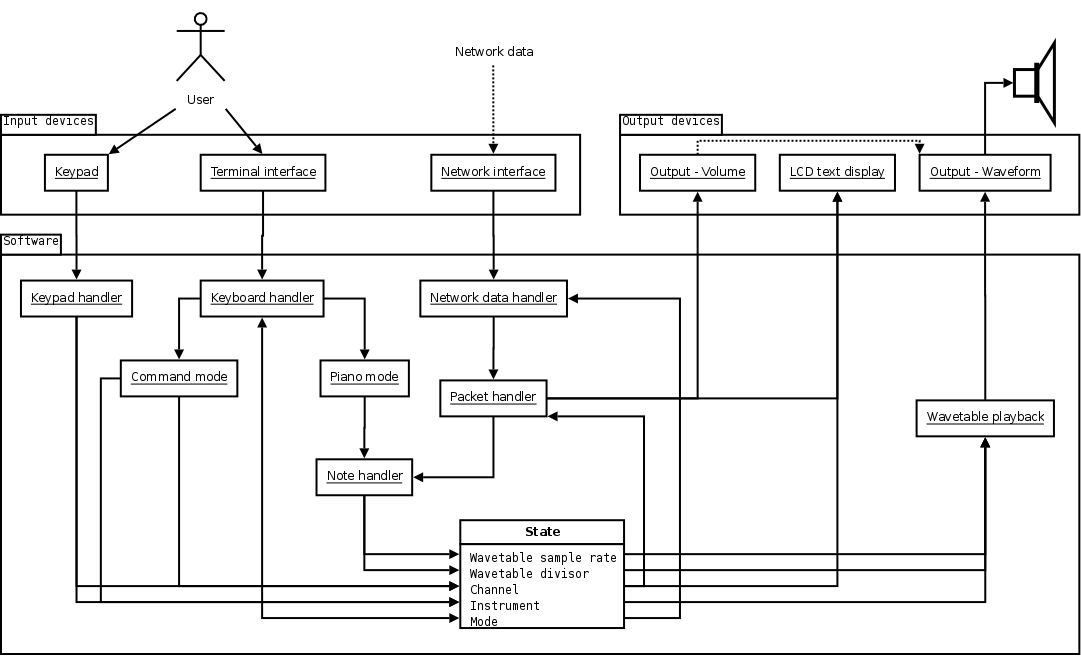
\includegraphics[totalheight=0.55\textheight,angle=90]{images/overview.png}
\caption{System overview}\label{fig:systemoverview}
\end{figure}

The diagram in Figure \ref{fig:systemoverview} shows the conceptual architecture of my system.  The 
basic idea is that various inputs are processed and in some way modify the state of the system, and 
this state in turn affects the operation of the continuously-running wave table playback.

The most important element of the system is the real-time conversion of network data to audio.  The 
network interface is a serial connection with a 19200bps baud rate.  Data arrives at a rate of one 
34-byte packet every 34ms.  The data format is sixteen pairs of bytes, each pair containing a MIDI 
note value and a volume level (both in the range 0-127), with each pair representing a channel 
between 0 and 15 (in order), and the packet is terminated with a null byte (0x00) and a carriage 
return (0x0D).  The mapping of channel identifiers to instruments is shown in Table 
\ref{tab:channelids}.  For the ``Percussion'' channel, the volume level represents the particular 
percussion instrument to play rather than the volume at which to play it.

\begin{table}[htbp]
\centering
\begin{tabular}[bp]{c l}
ID & Instrument \\
\hline
0 & Bass Guitar \\
1 & Cello \\
2 & Church Organ \\
3 & Piano \\
4 & Saxophone \\
5 & Melody \\
6 & Violin \\
7 & Trombone \\
8 & Trumpet \\
9 & French Horn \\
10 & Synth \\
11 & Electric Guitar \\
12 & Acoustic Guitar \\
13 & Flute \\
14 & Piccolo \\
15 & Percussion
\end{tabular}
\caption{Network data channels}\label{tab:channelids}
\end{table}

\subsection{Network}

% FIXME: contradiction with actual design?
The network handler deals with collecting data from the incoming bytes on the serial interface 
connected to the network and running the packet handler when the end of a packet is detected.  The 
carriage return is interpreted as the end of the packet, and the incoming bytes are counted and 
checked to detect and ignore incomplete packets.

When the end of a complete packet is detected, the packet handler is run.  The volume is converted 
from a 7-bit to 8-bit value and sent to the volume output, and also converted to hexadecimal and 
displayed on the LCD.  The MIDI note is used as the index in a lookup table for the PRT reload value 
and wave table divisor (see \ref{wavetables}), and also in another lookup table for a 4-character 
representation of the note which is shown on the LCD.

\subsection{Wave tables}
\label{wavetables}
% TODO: double check the maths!

In my design, all frequencies of the instruments are synthesised from the same wave table sample, 
therefore a way is needed to perform this frequency conversion.  A sample has two important 
interdependant properties - the sample rate and the frequency.  When changing either of these 
properties, the following property holds:

\begin{center}
${{F_{target}} \over {F_{source}}} = {{R_{target}} \over {R_{source}}}$
\end{center}

In other words, if a particular note is recorded at a particular sample rate, then the difference of 
the frequency when played is proportional to the sample rate it is played at.  In this case, we are 
aiming to play a particular frequency, so the required sample rate can be calculated with:

\begin{center}
${{R_{target}} = {{F_{target} \times {R_{source}}} \over {F_{source}}}}$
\end{center}

Unfortunately, at higher playback frequencies the necessary sample rate will be impractically high, 
so an additional way of changing the frequency is needed.  If for example only every other sample 
from the wave table is played, without changing the sample rate, this will double the frequency of 
the note being played, since the entire sample is being played twice as fast.  More generally, if a 
divisor $D$ is introduced, then ${F_{target}} = {F_{source} \times D}$.

To combine the two methods, $F_{target}$ can be replaced with ${F_{target}} \times D$.  With a 
little re-arrangement, the following equation can be obtained:

\begin{center}
${{R_{target}} \times D} = {{{F_{target} \times {R_{source}}} \over {F_{source}}}}$
\end{center}

See \ref{notelookuptables} for how this conversion is implemented to generate the MIDI note lookup 
tables.

\pagebreak
\section{Design and Implementation}

\subsection{Keypad handler}

The keypad is a slightly awkward device for trying to get a single value from - it interrupts the 
whole time that the key is being pressed.  When implementing the keypad handler, this was the main 
problem I had to overcome.

My solution was to create a kind of lockout for that particular interrupt handler.  The result is a 
variable that acts as an ``already handled'' flag for keypad interrupts.  When a keypad interrupt 
happens, the flag is checked - if it's non-zero, then the interrupt gets effectively ignored.  If 
it's zero, the interrupt handler executes as normal.  At the end of the interrupt handler, there are 
a few NOP instructions before setting the lockout variable back to zero and returning from the 
interrupt, but \emph{after} the interrupts are re-enabled.  The idea is that if the key is still 
pressed, it will interrupt during those NOPs, before the flag is cleared, and those interrupts will 
get ignored, but on the very last interrupt it will complete the handler.  This completely 
eliminates the possibility of accidental repeats.

For comparison, the alternative solution was to insert a delay after handling the keypress to allow 
time for the key to be released.  Unfortunately, that method was less than ideal, since if the delay 
was too long it would result in the system seeming unresponsive, and if too short then repeated 
interrupts would occur.  I felt it was better to maintain a direct responsiveness between action and 
reaction.

\subsection{Note lookup tables}
\label{notelookuptables}

Lookup tables are needed to contain the PRT value, divisor and note name (including octave) for 
every MIDI note.  The note names are in a separate lookup table to the other data as having an LCD 
information display was a lower priority than working sound playback and was implemented much later.

% TODO: expand on comparison of formats
The most efficient way to use a lookup value for a table is to multiply it by a power of two (left 
shifting), so blocks of data in the lookup table are also going to be $2^n$ bytes long.  However, 
the data for note playback is 3 bytes (a 16-bit PRT value plus an 8-bit divisor), so I was faced 
with the choice of having two lookup tables for the playback data or wasting $1\over4$ of the space 
used by the table.  After writing the necessary assembler for reading from both possible formats and 
analysing their execution times, I found that the single table method resulted in faster code.  
Combined with the fact I was not under pressure to conserve memory, I chose the single table method.

% TODO: expand on the result sorting
The Python script I wrote to generate the lookup tables ("tools/pitchtable.py") is based on the 
concept outlined in \ref{wavetables} for calculating the sample rates and divisors.  The actual 
method used involves working out the sample rate for every divisor between 1 and 255, removing all 
those resulting in a sample rate above 8kHz (a sensible maximum given the speed of the CPU), sorting 
the results in a way which tries to get the best combination of low error margin and high sample 
rate and using the first result (giving the PRT value and divisor).  The lookup table data format 
is:

\begin{center}
\begin{tabular}{c l}
Byte & Usage\\
\hline
0 & PRT value - Low byte\\
1 & PRT value - High byte\\
2 & Divisor\\
3 & Unused/null\\
\end{tabular}
\end{center}

The script also produces a second table which contains a 4-character representation of the note 
created from the octave number and note name.

The pitch table ("tools/pitchtable.csv") contains the octave numbers, MIDI note numbers, note names 
and frequencies in Comma-Separated Values format.  The Python script reads these in from standard 
input to generate the tables, which are written to standard output.

\pagebreak
\section{Testing and Evaluation}

\pagebreak
\section{Technical Specification}

\pagebreak
\section{Further Work}

% Merging the 2 MIDI lookup tables into one

\appendix

\pagebreak
\begin{thebibliography}{99}
% \bibitem{ref}Author:
% \emph{Title},
% \url{http://} (year)
\end{thebibliography}

\end{document}
